\documentclass{standalone}
\usepackage{tikz}
\usepackage{ctex,siunitx}
\setCJKmainfont{Noto Serif CJK SC}
\usepackage{tkz-euclide}
\usepackage{amsmath}
\usetikzlibrary{patterns, calc,3d}
\usetikzlibrary {decorations.pathmorphing,decorations.pathreplacing,decorations.shapes}
\begin{document}
\small
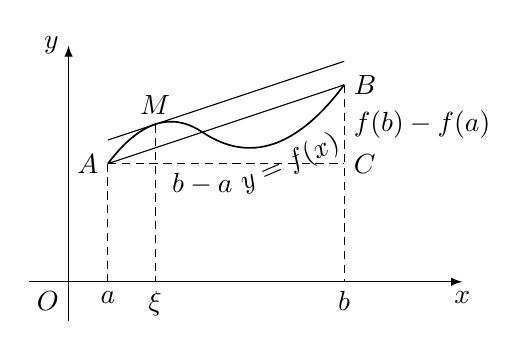
\begin{tikzpicture}[>=latex,scale=1.0]
  \draw[->](-0.5,0)--(5,0)node[below]{$x$};
  \draw[->](0,-0.5)--(0,3)node[left]{$y$};
  \draw[densely dashed](0.5,1.5)node[left]{$A$}--(0.5,0)node[below]{$a$}(1.1,2)node[above]{$M$}--(1.1,0)node[below]{$\xi$};
  \draw[densely dashed](3.5,2.5)node[right]{$B$}--(3.5,0)node[below]{$b$}(0.5,1.5)--(3.5,1.5)node[right]{$C$}node[pos=0.4,below]{$b-a$};
  \draw(0.5,1.5)--(3.5,2.5)(0.5,1.8)--(3.5,2.8);
  \draw[semithick](0.5,1.5)..controls(0.9,2.0333)and(1.3,2.1667)..(1.7,1.9)..controls(2.3,1.5)and(2.9,1.7)..(3.5,2.5)node[pos=0.55,below,sloped]{$y=f(x)$};
  \node at (3.5,2)[right]{$f(b)-f(a)$};
  % \draw[semithick,samples=200,domain=-1.2:1.8]plot(\x,{0.2*\x*\x*\x-0.3*\x*\x+0.3*\x});
  % \draw(0.5,1.5)--++(40:1.5)--({0.5+2.2*sqrt(3)},1.5)node[midway,above right=0.15]{$y=f(x)$};
  % \draw[densely dashed](0.5,1.5)--++(0,-1.5)node[below]{$a$}node[midway,right]{$f(a)$}({0.5+2.2*sqrt(3)},1.5)--++(0,-1.5)node[below]{$b$}node[midway,left]{$f(b)$}(0,1.5)node[left]{$k$}--({0.5+2.2*sqrt(3)},1.5);
  \node at (0,0)[below left]{$O$};
\end{tikzpicture}
\end{document}